\documentclass[12pt]{article}
\usepackage[left=2cm,right=2cm,top=2cm,bottom=2cm,letterpaper]{geometry}
\usepackage{lmodern}
\usepackage[T1]{fontenc}
\usepackage[utf8]{inputenc}
\usepackage[spanish,activeacute]{babel}
\usepackage{hyperref}
\usepackage{graphicx}
\graphicspath{{graphic/}}
\usepackage{float}
\usepackage{caption}
\usepackage[toc]{multitoc}
\setcounter{tocdepth}{2}
% automata
\usepackage{tikz}
\title{Proyecto 2}
\author{Carlos Gerardo Acosta Hernández \\ Andrea Itzel González Vargas \\ Luis Pablo Mayo Vega}
\date{Redes de Computadoras\\Facultad de Ciencias, UNAM}
%\setlength{\parindent}{0em}
\begin{document}
\maketitle
\tableofcontents
\newpage
\section{Especificación de requerimientos}
\subsection{Enunciado del problema}
De acuerdo con el modelo TCP/IP, \textit{la Capa de Aplicación} es la de mayor importancia y en la que se sustenta todo el desarrollo de redes de computadoras pues está compuesta por los protocolos y demás servicios encargados de manejar, intercambiar o decodificar los datos que los usuarios se envían a través de distintos hosts para comunicarse. En otras palabras, se busca que dos o más procesos en distintas computadoras puedan ser capaces de intercambiar información y de esta manera otorgar una mayor capacidad de procesamiento y mejor rendimiento del que se tendría con un único host.\\

Sin embargo, la \textit{Capa de Aplicación} no puede trabajar sola, siendo mediante un proceso de encapsulación en cada una de las capas, que los datos(PDU) se envian a las capas inferiores, añadiendo cada una de las capas información que le concierne para que sus protocolos puedan manejarlos.\\

Como sabemos, protocolos como \textsf{HTTP, DNS, FTP, SMTP o DHCP} tienen cada uno una estructura distinta ya bien definida y estandarizada en los articulos de \textit{Request for Comments} publicados, pero eso no significa que sean los únicos protocolos disponibles en la \textit{Capa de Aplicación}. La gran ventaja de esta capa es su adaptabilidad para que se desarrollen protocolos de acuerdo a las necesidades de la aplicación sobre la que se usarán. 

\subsection{Objetivo de la aplicación}

Esta aplicación fue creada con el objetivo de implementar un protocolo de la capa de aplicación en el que el usuario, conectado del lado del cliente, solicite un pokémon a capturar. El servidor elegirá aleatoriamente alguno de los pokémon que estén en su base de datos, se lo ofrecerá al usuario y, si éste acepta capturarlo, también aleatoriamente se indicará
 si logró capturarlo o no. \\

 El usuario también podrá ser capaz de consultar su Pokédex, con los nombres de los pokémon que ha capturado y la imagen de cada pokémon que seleccione. \\

 El protocolo que hemos diseñado se enfocará en las acciones del usuario y el servidor que involucren una comunicación entre ambos, cada una con un tipo de mensaje específico. Es decir, si un usuario quisiera capturar un pokémon, solo tendría que  enviar un mensaje con el código que el servidor entienda como "quiero capturar un pokémon" sin considerar otros aspectos como el nombre del pokémon o el tamaño de la imagen que contiene a tal pokémon. \\

 En ese sentido, diseñar nuestro propio protocolo nos permite tener mayor control sobre la tasa de transferencia de los datos dentro de la aplicación, disminuyendo los costos de la comunicación y mejorando el desempeño del programa.

 \newpage
 \subsubsection{Casos de uso}
 \begin{center}
   \begin{tabular}{|l|p{5cm}|p{9cm}|}
     \hline
     Actor & Caso de uso & Descripción \\
     \hline
     Pokentrenador & Iniciar sesión & El usuario se conecta con el servidor y se le muestra el menú principal de la aplicación \\ \hline
     Pokentrenador & Solicitar captura de pokémon & El usuario solicita al servidor que le muestre un pokémon para capturar \\ \hline
     Pokentrenador & Consultar pokedex & El usuario hace una consulta para buscar un pokémon en su pokédex \\ \hline
     Pokentrenador & Lanzar pokebola & El usuario intenta capturar el pokémon que le mostró el servidor, con un número de intentos límitado \\ \hline
     Pokentrenador & Cerrar sesión & Cierra la conexión con el servidor \\
     \hline
   \end{tabular}
 \end{center}
 \begin{figure}[H]
   \centering
   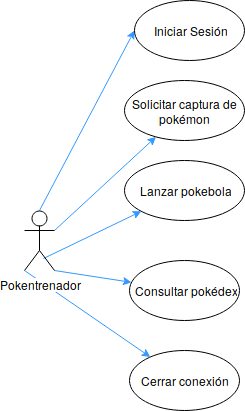
\includegraphics[width=0.4\textwidth]{casosdeuso}
   \caption{Diagrama de casos de uso de la aplicación}
 \end{figure}
 
\section{Diseño del protocolo}
\subsection{Máquina de Estados Finita}
Máquina de Estados Finita para el protocolo de la capa de aplicación.
\begin{center}
\begin{tikzpicture}[scale=0.2]
\tikzstyle{every node}+=[inner sep=0pt]
\draw [black] (7.7,-22) circle (3);
\draw (7.7,-22) node {$q_0$};
\draw [black] (21.9,-21.4) circle (3);
\draw (21.9,-21.4) node {$q_1$};
\draw [black] (35.4,-21.4) circle (3);
\draw (35.4,-21.4) node {$q_2$};
\draw [black] (63.3,-21.4) circle (3);
\draw (63.3,-21.4) node {$q_3$};
\draw [black] (35.4,-7.3) circle (3);
\draw (35.4,-7.3) node {$q_4$};
\draw [black] (63.3,-46.6) circle (3);
\draw (63.3,-46.6) node {$q_5$};
\draw [black] (35.4,-46.6) circle (3);
\draw (35.4,-46.6) node {$q_6$};
\draw [black] (7.7,-49.9) circle (3);
\draw (7.7,-49.9) node {$q_9$};
\draw [black] (9.968,-20.054) arc (121.77715:63.06187:9.706);
\fill [black] (19.48,-19.65) -- (18.99,-18.84) -- (18.54,-19.74);
\draw (14.59,-18.02) node [above] {$c:10$};
\draw [black] (24.9,-21.4) -- (32.4,-21.4);
\fill [black] (32.4,-21.4) -- (31.6,-20.9) -- (31.6,-21.9);
\draw (28.65,-21.9) node [below] {$s:20$};
\draw [black] (19.52,-23.209) arc (-61.01633:-114.14465:10.403);
\fill [black] (10.22,-23.6) -- (10.75,-24.39) -- (11.16,-23.47);
\draw (15,-25.09) node [below] {$s:44$};
\draw [black] (34.348,-24.204) arc (-26.53097:-150.98729:14.4);
\fill [black] (8.87,-24.76) -- (8.82,-25.7) -- (9.7,-25.21);
\draw (21.8,-32.71) node [below] {$c:11$};
\draw [black] (37.033,-9.805) arc (25.08093:-25.08093:10.722);
\fill [black] (37.03,-9.81) -- (36.92,-10.74) -- (37.82,-10.32);
\draw (38.54,-14.35) node [right] {$c:12$};
\draw [black] (34.029,-18.74) arc (-159.56755:-200.43245:12.574);
\fill [black] (34.03,-18.74) -- (34.22,-17.82) -- (33.28,-18.16);
\draw (32.74,-14.35) node [left] {$s:21/e:44$};
\draw [black] (38.4,-21.4) -- (60.3,-21.4);
\fill [black] (60.3,-21.4) -- (59.5,-20.9) -- (59.5,-21.9);
\draw (49.35,-21.9) node [below] {$c:13$};
\draw [black] (63.3,-24.4) -- (63.3,-43.6);
\fill [black] (63.3,-43.6) -- (63.8,-42.8) -- (62.8,-42.8);
\draw (62.8,-34) node [left] {$s:22$};
\draw [black] (38.199,-45.523) arc (108.58634:71.41366:34.985);
\fill [black] (38.2,-45.52) -- (39.12,-45.74) -- (38.8,-44.79);
\draw (49.35,-43.2) node [above] {$c:15$};
\draw [black] (60.488,-47.642) arc (-72.05358:-107.94642:36.146);
\fill [black] (60.49,-47.64) -- (59.57,-47.41) -- (59.88,-48.36);
\draw (49.35,-49.9) node [below] {$s:23$};
\draw [black] (35.4,-43.6) -- (35.4,-24.4);
\fill [black] (35.4,-24.4) -- (34.9,-25.2) -- (35.9,-25.2);
\draw (35.9,-34) node [right] {$s:24/e:41$};
\draw [black] (7.7,-25) -- (7.7,-46.9);
\fill [black] (7.7,-46.9) -- (8.2,-46.1) -- (7.2,-46.1);
\draw (7.2,-35.95) node [left] {$c:00$};
\draw [black] (61.07,-44.59) -- (37.63,-23.41);
\fill [black] (37.63,-23.41) -- (37.88,-24.32) -- (38.56,-23.58);
\draw (51.59,-33.51) node [above] {$c:14$};
\end{tikzpicture}
\end{center}


\subsection{Descripción de los estados}
\begin{center}
\begin{tabular}{|l|p{9cm}|}
  \hline
  Estado & Descripción \\
  \hline
  $q_0$ & Conexión establecida, inicio de aplicación. \\ \hline
  $q_1$ & Inicio de sesión. \\ \hline
  $q_2$ & Menú de juego. \\ \hline
  $q_3$ & Solicitud de captura de \textit{pókemon}. \\ \hline
  $q_4$ & Búsqueda de un pókemon en la \textit{pókedex}. \\ \hline
  $q_5$ & Aparición de un \textit{Pókemon} salvaje. \\ \hline
  $q_6$ & Intento de captura de \textit{pókemon}.\\ \hline
  $q_9$ & Cierre de conexión. \\
  \hline
\end{tabular}
\end{center}
\newpage

\subsection{Descripción de los mensajes en la comunicación cliente-servidor}
\begin{center}
  \begin{tabular}{|l|c|p{5.9cm}|}
    \hline
    Código & Segmento & Descripción \\ \hline
    \hline
    00 & \texttt{|code|num\_con|} & Termina la conexión identificada con num\_con. \\ \hline
    10 & \texttt{|code|num\_con|name|} & Solicitud de inicio de sesión del cliente. El parámetro \texttt{name} se refiere al nombre de usuario de la persona conectándose a través del cliente y su tamaño está en el rango de 1 a 32 bytes. \\ \hline
    11 & \texttt{|code|num\_con|} & Solicitud de cierre de sesión del cliente. \\ \hline
    12 & \texttt{|code|num\_con|name|} & Consulta del usuario a su \textit{Pokédex}. \\ \hline
    13 & \texttt{|code|num\_con|} & Menú de captura. \\ \hline
    14 & \texttt{|code|num\_con|} & El usuario rechaza el pokémon ofrecido aleatoriamente. \\ \hline
    15 & \texttt{|code|num\_con|} & Intento de captura del pokémon ofrecido aleatoriamente. \\ \hline
    20 & \texttt{|code|} & inicio de sesión exitoso. \\ \hline
    21 & \texttt{|code|long|nombre|longitud|imagen} & Pokédex query. \\ \hline %wat
    22 & \texttt{|code|name|num\_intentos\_restantes} & funcionamiento aleatorio. \\ \hline
    23 & \texttt{|code|} & Pokémon no capturado. \\ \hline
    24 & \texttt{|code| "2i"|} & Pokémon capturado. \\ \hline
    41 & \texttt{|code|} & Maximum Number of Attempts Reached. \\ \hline
    44 & \texttt{|code|} & Not Found Error. \\ \hline
    46 & \texttt{|code|} & No existe conexión. \\ \hline
    47 & \texttt{|code|} & Sin sesión. \\
    \hline
  \end{tabular}
\end{center}

\subsection{Diseño de la base de datos}
\section{Implementación del protocolo}
\subsection{Especificación del ambiente de desarrollo}

\subsection{Diagrama de clases (Maybe no, pero al menos mención de la estructura programática del proyecto, lo que sea más fácil jijijijijijij)}

\section{Uso y pruebas del protocolo}
\subsection{Manual de uso}
\subsection{Demostración del funcionamiento (por caso de uso ijijisjiajij)}

\end{document}
